\documentclass[graybox, envcountchap]{svmult}

% --- kodiranje, jezik, pisave -----------------------------------------
\usepackage[utf8]{inputenc}
\usepackage[T1]{fontenc}
\usepackage[slovene]{babel}
\usepackage{mathptmx}          % Times Roman
\usepackage{helvet}            % Helvetica
\usepackage{courier}           % Courier

% --- matematika -------------------------------------------------------
\usepackage{amsmath}
\usepackage{amssymb}
\usepackage{physics}           % \ket, \bra, \braket, \expval ...

% --- slike, tabele, diagrami ------------------------------------------
\usepackage{graphicx}
\usepackage{caption}
\usepackage{subcaption}
\usepackage{float}
\usepackage{booktabs}          % \toprule, \midrule, \bottomrule
\usepackage{multirow}
\usepackage{tabularx}
\usepackage[separate-uncertainty=true]{siunitx}
\sisetup{output-decimal-marker={,}}
\usepackage{tikz}
\usepackage{quantikz}          % kvantna vezja

% --- programska koda --------------------------------------------------
\usepackage{xcolor}
\usepackage{listings}
\lstset{
  basicstyle=\ttfamily\footnotesize,
  keywordstyle=\color{blue!60!black}\bfseries,
  commentstyle=\color{gray},
  stringstyle=\color{red!50!black},
  numbers=left, numberstyle=\tiny\color{gray},
  frame=single, breaklines=true, columns=fullflexible,
  showstringspaces=false, captionpos=b
}

% --- ostalo -----------------------------------------------------------
\usepackage{makeidx}
\usepackage{multicol}
\usepackage[bottom]{footmisc}
\usepackage{comment}
\usepackage{csquotes}          % \enquote{...}
\usepackage{import}            % \import{SkupinaXX/}{main}
\usepackage[numbers,square,sort&compress]{natbib} % številčni sklici [1--3]
\usepackage{xurl}
\usepackage[hidelinks]{hyperref}

\setlocalecaption{slovene}{theorem}{Izrek}
\setlocalecaption{slovene}{definition}{Definicija}


%%%%%%%%%%%%%%%%%%%%%%%%%%%%%%%%%%%%%%%%%%%%%%%%%%%%%%%%%%%%%%%%%%%%%%
% Skupina02/main.tex -- PRAZNO OGRODJE POGLAVJA
% Primer uporabe slik, tabel, enačb, vezij in kode je v Skupina01/main.tex.
%%%%%%%%%%%%%%%%%%%%%%%%%%%%%%%%%%%%%%%%%%%%%%%%%%%%%%%%%%%%%%%%%%%%%%

%%%% MOJA KODA %%%%

\graphicspath{{Skupina25/img/}}

\title{Implementacija in analiza reverzibilnih multiplekserjev na osnovi kvantnih celičnih avtomatov}
\author{Strahinja Ðorđević, Alja Eremić, Simona Cholakova}
\titlerunning{Reverzibilni multiplekserji v QCA}

\begin{document}
\maketitle

\abstract{V seminarju obravnavamo reverzibilne multiplekserje 2:1, 4:1 in 8:1, izvedene s tehnologijo kvantnih celičnih avtomatov (QCA). Predstavimo njihove osnovne gradnike, inverter in reverzibilna večinska vrata, ter pojasnimo načela njihovega delovanja in gradnje. Na podlagi vezij, predstavljenih v članku~\cite{alharbi2024}, v orodju QCADesigner-E izdelamo lastne implementacije multiplekserjev ter rezultate simulacij primerjamo z objavljenimi. Poleg tega predstavimo še lastno implementacijo reverzibilnega multiplekserja 16:1. Za vsa vezja analiziramo njihove glavne karakteristike, kot so površina, število celic in časovna zakasnitev, ter primerjamo njihove lastnosti.}

\section{Uvod}
\label{g25:sec:uvod}

[Motivacija: QCA kot alternativa CMOS, reverzibilna logika, vloga multiplekserja.
Sorodna dela.]

\begin{svgraybox}
\textbf{Raziskovalno vprašanje.} Ali lahko rezultate članka~\cite{alharbi2024}
potrdimo s ponovno izdelavo vezij in ali je mogoče zasnovo nadgraditi na
reverzibilni multiplekser 16:1?

\textbf{Pričakovani rezultat.} Ujemanje rezultatov simulacij za 2:1, 4:1 in 8:1
z rezultati, objavljenimi v članku \cite{alharbi2024}, ob predvidenih minimalnih odstopanjih, ter
delujoč multiplekser 16:1 z ocenjenimi lastnostmi.
\end{svgraybox}


\section{Osnovni gradniki}
\label{g25:sec:gradniki}

Reverzibilni multiplekser gradimo hierarhično. Najprej predstavimo osnovne gradnike: celice (razdelek~\ref{g25:sec:celica}), negator (razdelek~\ref{g25:sec:inverter}) in večinska vrata (razdelek~\ref{g25:sec:majority}). Iz njih zgradimo multiplekser 2:1 (razdelek~\ref{g25:sec:mux2}), ta pa nato služi kot gradnik za multiplekser 4:1 (razdelek~\ref{g25:sec:mux4}). Z nadaljnjim kombiniranjem teh modulov dobimo večja multiplekserja 8:1 (razdelek~\ref{g25:sec:mux8}) in 16:1 (razdelek~\ref{g25:sec:mux16}).

\subsection{Celica QCA in urino polje}
\label{g25:sec:celica}

Vsa vezja v QCA so sestavljena iz celic. Celica je kvadratna struktura s štirimi kvantnimi pikami in dvema elektronoma, ki se zaradi odbojne sile postavita v diagonalni konfiguraciji. Ti dve stanji, polarizaciji $P=-1$ in $P=+1$, kodirata logični vrednosti 0 in 1. Informacija se prenaša s coulombsko interakcijo med sosednjimi celicami in ne s tokom. Glede na vlogo ločimo tri vrste celic: vhodne, delovne in izhodne, ki so prikazane na sliki~\ref{g25:fig:cells}.

Prenos podatkov po vezju usmerja urino polje, ki ima štiri faze: preklop (angl.~\emph{switch}), zadržanje (angl.~\emph{hold}), sprostitev (angl.~\emph{release}) in mirovanje (angl.~\emph{relax}). Določa, kdaj celice sprejmejo vrednost, jo zadržijo in sprostijo.

\vspace{-0.7cm}
\begin{figure}[H]
\centering
\includegraphics[width=0.4\textwidth]{Skupina25/img/cells-1.png}
\caption{Vrste celic QCA: a) vhodna celica (modra), b) delovna celica (zelena) in c) izhodna celica (rumena).}
\label{g25:fig:cells}
\end{figure}

\subsection{Negator}
\label{g25:sec:inverter}

Prvi gradnik naših multiplekserjev je negator (angl.~\emph{inverter}),
ki izvaja funkcijo negacije: vhodno vrednost 0 preslika v 1 in vhodno
vrednost 1 v 0. Osnovna izvedba z eno vejo (angl.~\emph{single-branch
inverter}) je prikazana na sliki~\ref{g25:fig:inverter}a. V naših vezjih bomo uporabljali tudi negator z dvema vejama (angl.~\emph{double-branch
inverter}), prikazan na sliki~\ref{g25:fig:inverter}b.
Katero izvedbo izberemo, je odvisno od tega, koliko prostora imamo, kako
hitro mora vezje delovati in kako odporno mora biti na šum.

\begin{figure}[H]
\centering
\includegraphics[width=0.8\textwidth]{Skupina25/img/inverter-1.png}
\caption{Izvedbi negatorja v QCA: a) negator z eno vejo, b) negator z dvema vejama. Modra barva označuje vhodno celico, rumena izhodno celico, zelena pa notranje celice.}
\label{g25:fig:inverter}
\end{figure}

\subsection{Reverzibilna večinska vrata}
\label{g25:sec:majority}

Večinska vrata (angl. \emph{majority gate}) imajo tri vhode $A$, $B$ in $C$ ter en izhod $M(A,B,C)$, ki zavzame vrednost, ki se pojavi na vsaj dveh od treh vhodov:
\begin{equation}
    M(A,B,C) = AB + BC + AC .
\end{equation}
Ona nam bo omogocila da z njimi lahko izvedemo tako vrata IN (AND) kot vrata ALI (OR). Če je en vhod, na primer $C$, nastavljen na konstantno vrednost, se večinska vrata skrčijo na dvovhodna vrata:
\begin{align}
    M(A,B,0) &= A \ \text{AND} \ B, \\
    M(A,B,1) &= A \ \text{OR} \ B .
\end{align}

Skupaj z negacijo (NOT), ki je opisana v razdelku~\ref{g25:sec:inverter}, večinska vrata tvorijo poln nabor logičnih operacij.

Slika~\ref{g25:fig:majority}a prikazuje večinska vrata v QCA. Vhodni signali $A$, $B$ in $C$ se združijo v osrednji celici, ki zavzame polarizacijo, ki prevladuje med vhodi, ta pa se nato prenese na izhod $M(A,B,C)$.

Sliki~\ref{g25:fig:majority}b in~\ref{g25:fig:majority}c prikazujeta, kako isto strukturo uporabimo za izvedbo vrat AND in OR. Ker mora biti vezje reverzibilno, vhodov ne izgubimo, temveč jih na izhodu ohranimo v obliki kopij (\emph{A Copy} in \emph{B Copy}).
\begin{figure}[htbp]
    \centering
    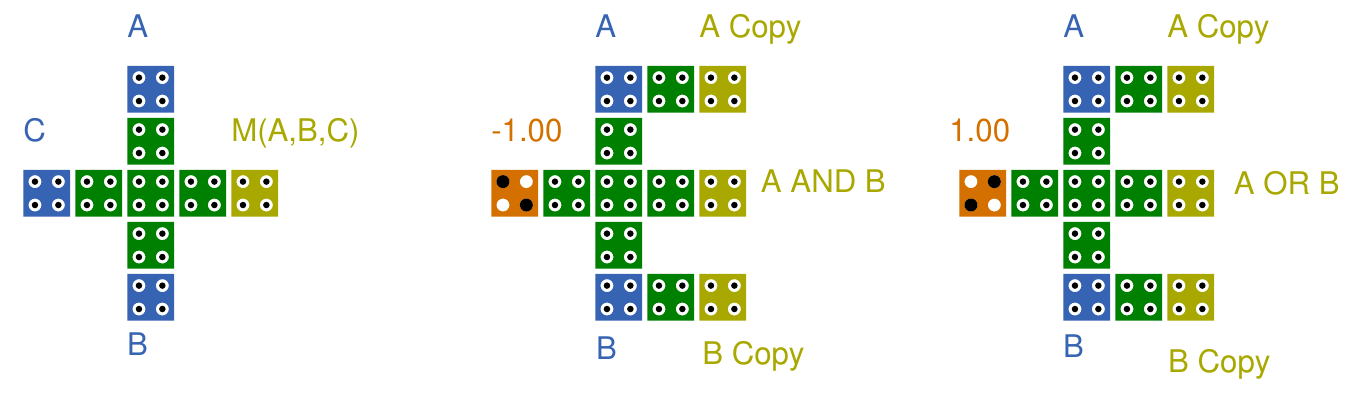
\includegraphics[width=\textwidth]{majority-1.png}
    \caption{Reverzibilna večinska vrata v QCA: a) večinska vrata $M(A,B,C)$, b) vrata AND z vhodom $C=-1$ ter c) vrata OR z vhodom $C=1$. Poleg rezultata sta na izhodu prisotni tudi kopiji vhodov $A$ in $B$.}
    \label{g25:fig:majority}
\end{figure}


\section{Metode}
\label{g25:sec:metode}

\subsection{Orodje in začetni parametri simulacije}
\label{g25:sec:orodja}
QCADesigner-E: velikost celice, razdalja med celicami, radij vpliva
(angl.~\emph{radius of effect}), ostali parametri (tabela).

\subsection{Zasnova poskusov}
\label{g25:sec:poskusi}
Ponovna izdelava vezij iz članka, vhodni vektorji, primerjava z objavljenimi
rezultati, nato lastna nadgradnja na 16:1.

\subsection{Metrike}
\label{g25:sec:metrike}
Površina, število celic, časovna zakasnitev (angl.~\emph{clock delay}).

\section{Zaporedna gradnja multiplekserjev}
\label{g25:sec:gradnja}

\subsection{Reverzibilni multiplekser 2:1}
\label{g25:sec:mux2}
Zgradba iz gradnikov (razdelek~\ref{g25:sec:gradniki}), lastnosti, zakasnitev.

\subsection{Reverzibilni multiplekser 4:1}
\label{g25:sec:mux4}
Kako uporabimo vezje 2:1; lastnosti, zakasnitev.

\subsection{Reverzibilni multiplekser 8:1}
\label{g25:sec:mux8}
Kako uporabimo vezji 2:1 in 4:1; lastnosti, zakasnitev.

\subsection{Reverzibilni multiplekser 16:1 (naša nadgradnja)}
\label{g25:sec:mux16}
Zasnova, razlike glede na 8:1; lastnosti, zakasnitev.

\section{Rezultati}
\label{g25:sec:rezultati}

\subsection{Primerjava z objavljenimi rezultati}
\label{g25:sec:primerjava}

\begin{table}[t]
\centering
\caption{Primerjava naših rezultatov z rezultati iz članka~\cite{alharbi2024}.}
\label{g25:tab:primerjava}
\begin{tabular}{lcccc}
\toprule
Vezje & Št.~celic & Površina & Zakasnitev & Vir \\
\midrule
2:1  & [ ] & [ ] & [ ] & članek \\
     & [ ] & [ ] & [ ] & naši \\
4:1  & [ ] & [ ] & [ ] & članek \\
     & [ ] & [ ] & [ ] & naši \\
8:1  & [ ] & [ ] & [ ] & članek \\
     & [ ] & [ ] & [ ] & naši \\
\bottomrule
\end{tabular}
\end{table}

\subsection{Lastnosti multiplekserja 16:1}
\label{g25:sec:lastnosti16}
Površina, zakasnitev, število celic.

\section{Razprava}
\label{g25:sec:razprava}

\subsection{Kaj ni delovalo}
\label{g25:sec:neuspehi}

\section{Zaključek}
\label{g25:sec:zakljucek}

\section*{Doprinosi avtorjev}
[ ]

\section*{Izjava o uporabi generativne umetne inteligence}
[ ]

%%%% KRAJ MOJE KODE %%%%

%%%% ZA BRISANJE %%%%
\backmatter
\bibliographystyle{unsrtnat}   % izpise tudi DOI in URL
\bibliography{references}
%%%%%%%%%%%%%%%%%%%%%

\end{document}
